\documentclass[twoside]{article}
\setlength{\oddsidemargin}{0.25 in}
\setlength{\evensidemargin}{-0.25 in}
\setlength{\topmargin}{-0.6 in}
\setlength{\textwidth}{6.5 in}
\setlength{\textheight}{8.5 in}
\setlength{\headsep}{0.75 in}
\setlength{\parindent}{0 in}
\setlength{\parskip}{0.1 in}

%
% ADD PACKAGES here:
%

\usepackage{amsmath}
\usepackage{amssymb}
%environment for proof
\usepackage{amsthm} 
%% package for hyperlinks,\href
\usepackage[colorlinks=true,allcolors=blue]{hyperref}
%figures packages
\usepackage{graphicx}
\usepackage{subcaption}
\usepackage[utf8]{inputenc}
\usepackage[export]{adjustbox}
%package for \toprule,\midrule,\bottomrule
\usepackage{booktabs} 

\usepackage{tikz}

%
% The following commands set up the lecnum (lecture number)
% counter and make various numbering schemes work relative
% to the lecture number.
%
\newcounter{lecnum}
\renewcommand{\thepage}{\thelecnum-\arabic{page}}
\renewcommand{\thesection}{\thelecnum.\arabic{section}}
\renewcommand{\theequation}{\thelecnum.\arabic{equation}}
\renewcommand{\thefigure}{\thelecnum.\arabic{figure}}
\renewcommand{\thetable}{\thelecnum.\arabic{table}}

%
% The following macro is used to generate the header.
%
\newcommand{\lecture}[4]{
	\pagestyle{myheadings}
	\thispagestyle{plain}
	\newpage
	\setcounter{lecnum}{#1}
	\setcounter{page}{1}
	\noindent
	\begin{center}
		\framebox{
			\vbox{\vspace{2mm}
				\hbox to 6.28in { { \it MANA130083.01 Nonparametric
						\hfill Spring 2025} }
				\vspace{4mm}
				\hbox to 6.28in { {\Large \hfill \bf Lecture #1 \hfill} }
				\vspace{2mm}
				\hbox to 6.28in { {\it Instructor: Prof. #3 \hfill Scribes: #4} }
				\vspace{2mm}}
		}
	\end{center}
	\markboth{Lecture #1: #2}{Lecture #1: #2}
}
%
% Convention for citations is authors' initials followed by the year.
% For example, to cite a paper by Leighton and Maggs you would type
% \cite{LM89}, and to cite a paper by Strassen you would type \cite{S69}.
% (To avoid bibliography problems, for now we redefine the \cite command.)
% Also commands that create a suitable format for the reference list.
\renewcommand{\cite}[1]{[#1]}
\def\beginrefs{\begin{list}%
		{[\arabic{equation}]}{\usecounter{equation}
			\setlength{\leftmargin}{2.0truecm}\setlength{\labelsep}{0.4truecm}%
			\setlength{\labelwidth}{1.6truecm}}}
	\def\endrefs{\end{list}}
\def\bibentry#1{\item[\hbox{[#1]}]}

%Use this command for a figure; it puts a figure in wherever you want it.
%usage: \fig{NUMBER}{SPACE-IN-INCHES}{CAPTION}
\newcommand{\fig}[3]{
	\vspace{#2}
	\begin{center}
		Figure \thelecnum.#1:~#3
	\end{center}
}
% Use these for theorems, lemmas, proofs, etc.
\newtheorem{theorem}{Theorem}
\newtheorem*{theorem*}{Theorem}
\newtheorem{proposition}{Proposition}
\newtheorem{assumption}{Assumption}
\newtheorem{corollary}{Corollary}
\newtheorem*{corollary*}{Corollary}
\newtheorem*{example*}{Example}
\newtheorem{lemma}{Lemma}
\newtheorem*{lemma*}{Lemma}
\newtheorem{definition}{Definition}
\newtheorem*{definition*}{Definition}
% **** IF YOU WANT TO DEFINE ADDITIONAL MACROS FOR YOURSELF, PUT THEM HERE:

\newcommand\E{\mathbb{E}}

\begin{document}
	%FILL IN THE RIGHT INFO.
	%\lecture{**LECTURE-NUMBER**}{**DATE**}{**LECTURER**}{**SCRIBE**}
	\lecture{4}{Mar.12}{Bowen Gang}{Yize Wang, Jingyi Zhou}
	%\footnotetext{These notes are partially based on those of Nigel Mansell.}
	
	% **** YOUR NOTES GO HERE:
	
	% Some general latex examples and examples making use of the
	% macros follow.
	%**** IN GENERAL, BE BRIEF. LONG SCRIBE NOTES, NO MATTER HOW WELL WRITTEN,
	%**** ARE NEVER READ BY ANYBODY.
	\section{Review: Kolmogorov-Smirnov Two Sample Test}
	Consider the basic setup: we have observations $X_1, ..., X_m \sim F_X$ and $Y_1, ..., Y_n \sim F_Y$. The null hypothesis is $F_X = F_Y$. The K-S statistic is given by
	$$
	D_{m,n} = \max_{x} |\hat{F}_X(x) - \hat{F}_Y(x)|
	$$
	where we reject the null when $D_{m,n} > d$ for some $d$. In order to calculate the p-value $\Pr \left( D_{m,n} > d | H_0 \right)$, we can either do simulation or use the following formula. To derive the exact formula, we do the following process. We combine the two series of observations together and rank them from smallest to largest. This sequence corresponds to a 'path' from the grid (0,0) to (m,n). Say the sequence is $X_{(1)}, X_{(2)}, Y_{(1)}, Y_{(2)}, X_{(3)}, Y_{(3)}, X_{(4)}, Y_{(4)}$. We may draw the following path, where $X$ moves the point to rightward and $Y$ moves the point upward. 
	\begin{center}
		\begin{tikzpicture}[domain=0:5]
			\draw[->](-0.2,0) -- (5.2,0) node[below] {};
			\draw[->](0,-0.2) -- (0, 5.2) node[below] {};
			\draw[very thin, color=green] (0,0) grid (5,5);
			\draw[domain = 0:2] plot(\x, 0);
			\draw[domain = 0:2] plot(2, \x);
			\draw[domain = 2:3] plot(\x, 2);
			\draw[domain = 2:3] plot(3, \x);
			\draw[domain = 3:4] plot(\x, 3);
			\draw[domain = 3:4] plot(4, \x);
		\end{tikzpicture}
	\end{center}
	Then all the observed values of $m \hat{F}_X(x)$ and $n \hat{F}_Y(x)$ are respectively the coordinates of all points $(u,v)$ on the path. There are $\binom{m+n}{n}$ possible paths in total. We are actually trying to find $\max |\frac{u}{m} - \frac{v}{n}| = \frac{|nu-mv|}{mn}$, which is equivalent to $\max |\hat{F}_X(x) - \hat{F}_Y(x)|$. We then link the origin point and $(m,n)$ in the graph: 
	\begin{center}
		\begin{tikzpicture}[domain=0:5]
			\draw[->](-0.2,0) -- (5.2,0) node[below] {};
			\draw[->](0,-0.2) -- (0,5.2) node[below] {};
			\draw[very thin, color=green] (0,0) grid (5,5);
			\draw[domain = 0:2] plot(\x, 0);
			\draw[domain = 0:2] plot(2, \x);
			\draw[domain = 2:3] plot(\x, 2);
			\draw[domain = 2:3] plot(3, \x);
			\draw[domain = 3:4] plot(\x, 3);
			\draw[domain = 3:4] plot(4, \x);
			\draw[dashed, domain = 0:4] plot(\x, \x);
		\end{tikzpicture}
	\end{center}
	where the dashed line is given by $nx-my=0$. Further, the vertical distance between $(u,v)$ and $nx-my=0$ is given by
	$$
	\left| v - \frac{nu}{m} \right|
	$$
	Let $\frac{\left| nu-mv \right|}{mn} = d$, it is obvious that
	$$
	\left| v - \frac{nu}{m} \right| = nd
	$$
	Then the p-value is equivalent to calculate the number of paths whose distances from the dashed line are less than or equal to $nd$. The total number of path is given by $\binom{m+n}{n}$. Again we want to compute the number of paths which have points at a distance from the diagonal not less than $nd$. Let $A(m,n)$ be the number of paths from $(0,0)$ to $(m,n)$ which lie entirely within the boundary lines, where the distances between each boundary line and the dashed line is $nd$. 
	\begin{center}
		\begin{tikzpicture}[domain=0:5]
			\draw[->](-0.2,0) -- (5.2,0) node[below] {};
			\draw[->](0,-0.2) -- (0,5.2) node[below] {};
			\draw[very thin, color=green] (0,0) grid (5,5);
			\draw[dashed, domain = 0:4] plot(\x, \x);
			\draw[dashed, domain = 0:2.5] plot(\x, \x + 1.5);
			\draw[dashed, domain = 1.5:4] plot(\x, \x - 1.5);
		\end{tikzpicture}
	\end{center}
	Then
	$$
	Pr \left( D_{m,n} > d | H_0 \right) = 1 - \frac{A(m,n)}{\binom{m+n}{n}}
	$$
	Note that we have the recursive formula
	$$
	A(u,v) = A(u-1, v) + A(u, v-1)
	$$
	where the initial condition is given by: 
	$$
	A(0, v) = A(u, 0) = 1
	$$
	Then the exact distribution of K-S two sample test is solved. 

	
	\section{The Median Test}
	The basic setting is still $X_1, ..., X_m \sim F_X$ and $Y_1, ..., Y_n \sim F_Y$. We are interested in the question that $F_X = F_Y$. The naive idea is that under this null, the two samples should have similar distributions. To be more specific, let 
	$$
	P_X = Pr \left( X \leqslant \delta \right) \; and \; P_Y = Pr \left( Y \leqslant \delta \right)
	$$
	then under $H_0$ we have $P_X = P_Y$. Also let $u$, $v$ be the respective number of $X$ and $Y$ observations less than $\delta$. If $u$ and $v$ are far away from each other, we tend to reject the null. The joint distribution of $U, V$ is given by
	$$
	f_{U,V}(u,v) = \binom{m}{u} P_X^u \left( 1 - P_X \right)^{m-u} \cdot \binom{n}{v} P_Y^v \left( 1 - P_Y \right)^{n-v}
	$$
	Under $H_0$, $P_X = P_Y = p$. We can estimate $p$ by calculate $\frac{u+v}{m+n}$. If you take $\delta$ to be the median of the combined sample, we tend to reject the null when $u$ differs significantly from $\frac{m}{2}$. To be more specific, let $N=m+n$ and the median $t$ is given by
	\begin{align*}
		t = \begin{cases}
			\frac{N}{2}, \; &if \; N \; even \\
			\frac{N+1}{2}, \; &if \; N \; odd
		\end{cases}
	\end{align*}
	The test statistic is then given by
	$$
	Z = \frac{U - \frac{mt}{N}}{\left( mnt (N-t) / N^3 \right)^{\frac{1}{2}}} \xrightarrow{H_0} N(0,1)
	$$
	In order to show the result explicitly, we do the following process: 
	\begin{align*}
		z &= \frac{Nu - mt}{\sqrt{mnt(N-t)/N}} \\
		&= \frac{nu - m(t-u)}{\sqrt{mnN \left( \frac{t}{N} \right) \left( 1 - \frac{t}{N} \right)}} \\
		&= \frac{\frac{u}{m} - \frac{v}{n}}{\sqrt{\left( \frac{u+v}{N} \right) \left( 1 - \frac{u+v}{N} \right) \frac{N}{mn}}} \\
		&\approx \frac{\frac{u}{m} - \frac{v}{n}}{\sqrt{\hat{p} \left( 1 - \hat{p} \right) \left( \frac{1}{m} + \frac{1}{n} \right)}} \rightarrow N(0,1)
	\end{align*}
	Note that there is an extra incremental randomness here: we do not know the median at first. We estimate the median by using pooled sample median. 
	
	\section{The Control Median Test}
	The basic setup is still based on $X_1, ..., X_m \sim F_X$ and $Y_1, ..., Y_n \sim F_Y$ and we want to test $H_0: F_X = F_Y$. Here we let
	$$
	V = \# \; of \; X \; less \; than \; the \; median \; of \; Y
	$$
	where we tend to reject the null if $v$ differs from $\frac{m}{2}$ too much. For simplicity, we assume $n$ is odd: $n = 2r+1$ then
	$$
	Pr \left[ V=j | H_0 \right] = \frac{\binom{m+r-j}{m-j} \binom{j+r}{j}}{\binom{m+2r+1}{m}}
	$$
	In practice, we use the following approximation instead: 
	$$
	z = \frac{v - \frac{m}{2}}{\sqrt{m(m+n)/4n}} \xrightarrow{D} N(0,1)
	$$
	
	\section{The Mann Whitney U Test}
	Let $U = \#$ of times a $Y$ proceeds an $X$ in the combined ordered arrangement of two independent random samples $X_1, ..., X_m$ and $Y_1, ..., Y_n$. To be more specific, let
	\begin{align*}
		D_{ij} = \begin{cases}
			1, \; if \; Y_j < X_i \\
			0, \; if \; Y_j > X_i
		\end{cases}
	\end{align*}
	then the test statistic is given by
	$$
	U = \sum_{i=1}^{m} \sum_{j=1}^{n} D_{ij}
	$$
	For example, the ordered sample is 
	$$
	X_{(1)}, X_{(2)}, Y_{(1)}, Y_{(2)}, X_{(3)}, Y_{(3)}, X_{(4)}
	$$
	Here are two $X$'s that proceed $Y_{(1)}$ and $Y_{(2)}$ and one $X$ that proceeds $Y_{(3)}$. So $U = 2+2+1=5$. You can imagine that if $X$ and $Y$ has different distributions, say $F_X > F_Y$ or $F_Y < F_X$, $U$ will be either too small or too large: 
	\begin{align*}
		X_{(1)}, X_{(2)}, X_{(3)}, X_{(4)}, Y_{(1)}, Y_{(2)}, Y_{(3)} \tag{U=0} \\
		Y_{(1)}, Y_{(2)}, Y_{(3)}, X_{(1)}, X_{(2)}, X_{(3)}, X_{(4)} \tag{U=12}
	\end{align*}
	So what is the null distribution of $U$? Under null hypothesis, 
	$$
	f_U(u) = Pr \left( U = u \right) = \frac{r_{m,n}(u)}{\binom{m+n}{n}}
	$$
	where $r_{m,n}(u)=\#$ of distinguishable arrangements such that in each sequence the $\#$ of times a $Y$ proceeds an $X$ is exactly $u$. We can calculate $r_{m,n}(u)$ recursively: 
	$$
	r_{m,n}(u) = r_{m,n-1}(u) + r_{m-1,n}(u-n)
	$$
	where the initial condition is given by
	\begin{align*}
		\begin{cases}
			r_{i,j}(u) = 0, &\forall u < 0 \\
			r_{i,0}(0) = 1, \\
			r_{0,i}(0) = 1, \\
			r_{i,0}(u) = 0, &\forall u \neq 0 \\
			r_{0,i}(u) = 0, &\forall u \neq 0
		\end{cases}
	\end{align*}
	Now we have solved the exact distribution and we will derive the asymptotic distribution as follows. Let
	$$
	p = Pr \left( Y < X \right)
	$$
	then
	\begin{align*}
		\mathbb{E} \left[ D_{ij} \right] &= p = \mathbb{E} \left[ D_{ij}^2 \right] \\
		Var \left[ D_{ij} \right] &= p(1-p) \\
		Cov \left[ D_{ij}, D_{hk} \right] &= 0 \; for \; i \neq h, j \neq k \\
		Cov \left[ D_{ij}, D_{ik} \right] &= \underbrace{\mathbb{E} \left[ D_{ij}D_{ik} \right]}_{0-1 \; variable} - \underbrace{\mathbb{E} \left[ D_{ij} \right] \mathbb{E} \left[ D_{ik} \right]}_{p^2}
	\end{align*}
	where we can also let
	$$
	p_1 = \mathbb{E} \left[ D_{ij}D_{ik} \right] = Pr \left( Y_j < X_i \cap Y_k < X_i \right)
	$$
	Similarly
	$$
	Cov \left[ D_{ij}, D_{hj} \right] = p_2 - p^2
	$$
	where
	$$
	p_2 = Pr \left( X_i > Y_j \cap X_h > Y_j \right) = \mathbb{E} \left[ D_{ij} D_{hj} \right]
	$$
	In order to calculate $p_1$ and $p_2$, we can do the following integration: 
	\begin{align*}
		p_1 &= Pr \left( Y_j < X_i \; and \; Y_k < X_i \right) \\
		&= Pr \left( Y_j \; \mathrm{and} \; Y_k < X_i \right) \\
		&= \mathbb{E}_{X_i} \Pr \left( Y_j \; \mathrm{and} \; Y_k < X_i | X_i \right) \\
		&= \mathbb{E}_{X_i} [F(X_i)]^2 \\
		&= \int_{- \infty}^{\infty} \left[ F_Y(x) \right]^2 \underbrace{d F_X(x)}_{f_X(x)dx}
	\end{align*}
	Under the null, $F_Y(x) = F_X(x)$ thus
	\begin{align*}
		\int_{- \infty}^{\infty} \left[ F_Y(x) \right]^2 d F_X(x) &= \int_{- \infty}^{\infty} \left[ F_X(x) \right]^2 d F_X(x) \\
		&= \frac{1}{3}
	\end{align*}
	Similarly
	$$
	p_2 \stackrel{H_0}{=} \frac{1}{3}
	$$
	Finally we have
	\begin{align*}
		\mathbb{E} \left[ U \right] &= \sum_{i=1}^{m} \sum_{j=1}^{n} \mathbb{E} \left[ D_{ij} \right] = mnp \\
		Var \left[ U \right] &= \sum \sum Var \left[ D_{ij} \right] + \sum \sum \sum \sum Cov \left[ D_{ij}, D_{hk} \right] \to mn[p - p^2 (N-1) + (n-1) \frac{1}{3} + (m-1) \frac{1}{3}] \\
		&= \frac{mn(N+1)}{12} \quad (\mathrm{under} \; H_0, p = \frac{1}{2})
	\end{align*}
	where $N = m+n$. And the normalized distribution is asymptotically normal: 
	$$
	Z = \frac{U - \frac{mn}{2}}{\sqrt{\frac{mn(N+1)}{12}}} \rightarrow N(0,1)
	$$
	If we have ties in our observations, say, $X_i = Y_j$, we can think about using a modified test: 
	\begin{align*}
		D_{ij}^{\star} = \begin{cases}
			1, &if \; X_i > Y_j \\
			0, &if \; X_i = Y_j \\
			-1, &if \; X_i < Y_j
		\end{cases}
	\end{align*}
	and similarly
	$$
	U = \sum \sum D_{ij}^{\star}
	$$
	
	\section{Linear Rank Statistics}
	\subsection{Definition}
	The basic setup is still: $X_1, ..., X_m \sim F_X$ and $Y_1, ..., Y_n \sim F_Y$. The null hypothesis is $F_X = F_Y$. For linear rank statistic, we need to construct vector $z$, where
	$$
	z = \left( z_1, z_2, ..., z_N \right), N=m+n
	$$
	For each element of $z$, 
	\begin{align*}
		z_i = \begin{cases}
			1, &if \; i^{th} \; sample \; is X \\
			0, &if \; i^{th} \; sample \; is Y
		\end{cases}
	\end{align*}
	where we actually mean combined ordered sample we we say 'sample' here. For example, if
	\begin{align*}
		(X_1, X_2, X_3, X_4) = (2, 9, 3, 4) \\
		(Y_1, Y_2, Y_3) = (1,6,10)
	\end{align*}
	then the combined ordered sample is given by
	\begin{align*}
		1, 2, 3, &4, 6, 9, 10 \\
		Y_1, X_1, X_3, &X_4, Y_2, X_2, Y_3 
	\end{align*}
	and the corresponding $z$ is
	$$
	z = (0, 1, 1, 1, 0, 1, 0)
	$$
	Linear rank statistic is  a statistic of the form
	$$
	T_N(z) = \sum_{i=1}^{N} a_i z_i
	$$
	
	\subsection{Properties of Linear Rank Statistic}
	\begin{theorem*}
		Under $H_0: F_X=F_Y$, we have
		\begin{align*}
			\mathbb{E} \left[ z_i \right] &= \frac{m}{N}, \; Var \left[ z_i \right] = \frac{mn}{N^2} \\
			cov \left[ z_i, z_j \right] &= \frac{-mn}{N^2 (N-1)}
		\end{align*}
	\end{theorem*}
	The proof is immediate from $z_i \sim Ber \left( \frac{m}{N} \right)$. For the covariance, 
	\begin{align*}
		cov \left[ z_i, z_j \right] &= \mathbb{E} \left[ z_i z_j \right] - \mathbb{E} \left[ z_i \right] \mathbb{E} \left[ z_j \right] \\
		&= Pr \left( z_i = 1 \& z_j = 1 \right) - \left( \frac{m}{N} \right)^2 \\
		&= \frac{\binom{m}{2}}{\binom{N}{2}} - \left( \frac{m}{N} \right)^2 \\
		&= \frac{m(m-1)}{N(N-1)} - \left( \frac{m}{N} \right)^2 \\
		&= \frac{-mn}{N^2 (N-1)}
	\end{align*}
	\begin{theorem*}
		Under $H_0$, 
		\begin{align*}
			\mathbb{E} \left[ T_N \right] &= m \sum \frac{a_i}{N} \\
			Var \left[ T_N \right] &= \frac{mn}{N^2 (N-1)} \left[ N \sum_{i=1}^{N} a_i^2 - \left( \sum_{i=1}^{N} a_i \right)^2 \right]
		\end{align*}
	\end{theorem*}
	The proof is immediate from 
	\begin{align*}
		\mathbb{E} \left[ T_N \right] &= \mathbb{E} \left[ z_i \right] \sum a_i \\
		Var \left[ T_N \right] &= Var \left( \sum a_i z_i \right) = \sum a_i^2 Var \left[ z_i \right] + \mathop{\sum\sum}\limits_{i \neq j} a_i a_j cov \left[ z_i, z_j \right]
	\end{align*}
	\begin{theorem*}
		If $B_N = \sum_{i=1}^{N}$, $T_N = \sum_{i=1}^{N}a_i z_i$, then
		\begin{align*}
			cov\left( B_N, T_N \right) = \frac{mn}{N^2 (N-1)} \left[ N \left(\sum a_i b_i \right) - \left( \sum a_i \right) \left( \sum b_i \right) \right]
		\end{align*}
	\end{theorem*}
	The proof is also immediate because both $B_N$ and $T_N$ are linear rank statistics, which can be seen as $\vec{a} \cdot \vec{z}$.
	\begin{definition*}
		$T_N(z)$ is symmetric if 
		\begin{align*}
			Pr \left[ T_N(z) - \mu = k \right] = Pr \left[ T_N (z) - \mu = -k \right]
		\end{align*}
		where $\mu = \mathbb{E} \left[ T_N(z) \right]$. This definition is actually: the p.m.f. is symmetric. 
	\end{definition*}
	The question is, how can we tell a linear rank statistic is symmetric? Suppose we observe that for every $z$, a conjugate $z'$ exists s.t. whenever $T_N(z) = \mu + k$, we have $T_N(z') = \mu - k$. Then the frequency of $T_N(z) = \mu+k$ is the same as that of $\mu - k$ (i.e., $T_N(z')$). So the distribution is symmetric. The condition for symmetry is then $T_N(z) + T_N(z') = 2 \mu$. Similarly we have the following theorem. 
	\begin{theorem*}
		The null distribution of $T_N(z)$ is symmetric about $\mu$ whenever $a_i + a_{N-i+1} = c$ for $i = 1, 2, ..., N$, where $a_i$ can be seen as a weight of $z_i$. 
	\end{theorem*}
	The proof is as follows: given $z = (z_1, z_2, ..., z_N)$, let $z' = (z_1', z_2', ..., z_N')$, where $z_i' = z_{N-i+1}$ . Then you can verify that 
	\begin{align*}
		T_N(z) + T_N(z') &= \sum a_i z_i + \sum a_i z_{N-i+1} \\
		&= \sum_{i=1}^{N} a_i z_i + \sum_{j=1}^{N} a_{N-j+1}z_j \\
		&= \sum_{j=1}^{N} \left( a_i + a_{N-j+1} \right) z_j \\
		&= c \sum z_j = cm \; (constant)
	\end{align*}
	\begin{theorem*}
		The null distribution of $T_N(z)$ is symmetric about its mean for any wet of weight if $m=n=\frac{N}{2}$. 
	\end{theorem*}
	The proof is also to find a conjugate. Define conjugate $z'$ with $z_i' = 1 - z_i$. Then
	\begin{align*}
		T_N(z) + T_N(z') &= \sum a_i z_i + \sum a_i (1-z_i) \\
		&= \sum a_i z_i + \sum a_i - \sum a_i z_i = \sum a_i \; (constant)
	\end{align*}
	\begin{theorem*}
		The null distribution of $T_N(z)$ is symmetric about its mean if $N$ is even and the weights are $a_i = i$ for $i \leqslant \frac{N}{2}$ and $a_i = N-i+1$ for $i > \frac{N}{2}$. 
	\end{theorem*}
	That is to say, $a = (1, 2, ..., \frac{N}{2}, \frac{N}{2}, \frac{N}{2} - 1, \frac{N}{2} - 2, ..., 3, 2, 1)$. The proof is similar as previous ones. In practice, we also use the following asymptotic distribution a lot. 
	\begin{align*}
		\frac{T_N \left( z \right) - \mathbb{E} \left[ T_N(z) \right]}{\sqrt{Var \left[ T_N(z) \right]}} \to N(0,1)
	\end{align*}

	\subsection{Linear Rank Tests for the Location Problem}
	For this part, the null is given by $F_X=F_Y$ and the alternative hypothesis is given by $F_Y(x) = F_X(x - \theta)$ where $\theta \neq 0$. This is a shift of location and that is why it is called as a location problem/test. In parametric context, if $F$ is normal, we use t-test. In non-parametric case, we can use the Wilcoxon rank sum test. The test statistic is given by
	\begin{align*}
		W_N = \sum_{i=1}^{N} i z_i
	\end{align*}
	We will reject the null if $W_N$ is too big or too small. This is a type of linear rank statistic where the weight is $a_i = i$. It is symmetric because here we have $a_i = a_{N-i+1} = c$. We also know its asymptotic distribution. 
	\subsubsection{The Exact Distribution of Wilcoxon Rank Sum Statistic}
	Let $r_{m,n}(k) = \#$ of arrangements of $m*X$ and $n*Y$ s.t. the sum of $X$ rank is $k$. Then
	\begin{align*}
		r_{m,n}(k) = \underbrace{r_{m-1, n}(k-N)}_{N^{th} \; position \; is \; X} + \underbrace{r_{m,n-1}(k)}_{N^{th} \; position \; is \; Y} 
	\end{align*}
	This recursive process is quite similar to that of Mann Whitney U test ($r_{m,n}(u) = r_{m,n-1}(u) + r_{m-1, n}(u-n)$. You can actually prove that they are equivalent. Recall the Mann Whitney U statistics is given by $U = \sum_{i=1}^{m} \sum_{j=1}^{n} D_{ij}$, which is equal to 
	\begin{align*}
		\sum_{i=1}^{m} \underbrace{\left( D_{i1} + D_{i2} + \cdots + D_{in} \right)}_{\# \; of \; values \; of \; j \; for \; which \; Y_j<X_i}
	\end{align*}
	which can also be considered as the rank of $X_i$ reduced by $n_i$ where $n_i = \#$ of $X's \leqslant X_i$.  Then
	\begin{align*}
		U &= \sum_{i=1}^{m} \sum_{j=1}^{n} D_{ij} \\
		&= \sum_{i=1}^{m} \left( r(X_i) - n_i \right) \\
		&= \sum_{i=1}^{m} r \left( X_i \right) - \underbrace{\left( n_1 + n_2 + \cdots + n_m \right)}_{permutation \; of \; 1,2,...,m} \\
		&= \sum_{i=1}^{m} r \left( X_i \right) - \left( 1 + 2 + \cdots + n_m \right) \\
		&= \sum_{i=1}^{m} \underbrace{r \left(X_i \right)}_{\sum i z_i} - \underbrace{\frac{m}{2}(m+1)}_{constant}
	\end{align*}
	So the Mann Whitney U statistic and the Wilcoxon rank sum test only differ by a constant. 
	\subsubsection{Terry-Heffding (Normal Scores) Test}
	Here the test statistic is given by 
	\begin{align*}
		\sum_{i=1}^{N} \mathbb{E} \left[ \xi_{(i)} \right] z_i
	\end{align*}
	where $\xi_i$ is the $i^{th}$ order statistic of standard normal distribution. If $F_X$ and $F_Y$ happen to follow normal distribution, $H_0: F_X= F_Y \sim N(\mu, \sigma^2)$ and $H_a: F_X \sim N(\mu_1, \sigma^2), F_Y \sim N(\mu_2, \sigma^2)$, then the Terry-Hoeffding is asymptotically optimal, which means it will have higher power than other rank tests. This is because $\mathbb{E} \left[ \xi_{(i)} \right]$ is "more representative" of the raw data than the rank. To be more specific, 
	\begin{align*}
		corr \left( \mathbb{E} \left[ \xi_{(i)} \right], X_i \right) \geqslant corr \left( i, X_i \right)
	\end{align*}
	The pitfall of Terry-Hoeffding is that it is difficult to compute $\mathbb{E} \left[ \xi_{(i)} \right]$. Then we can replace the test statistic by
	\begin{align*}
		\sum_{i=1}^{N} \Phi^{-1} \left( \frac{i}{N+1} \right) z_i
	\end{align*}
	where $\Phi(\cdot)$ is the CDF for $N(0,1)$ and $\frac{i}{N+1}$ can be seen as a quantile. Then $\Phi^{-1} \left( \frac{i}{N+1} \right)$ can be viewed as an approximate of $\mathbb{E} \left[ \xi_{(i)} \right]$. 
	
\end{document}